\documentclass[a4paper]{article}
\usepackage{authblk}
\usepackage[backend=bibtex]{biblatex}
\usepackage{hyperref}
\usepackage{txfonts}
\usepackage{titling}
\usepackage{graphicx}
\usepackage{subcaption}
\usepackage[a4paper, margin={2.5cm, 1.7cm}]{geometry}
\usepackage{mwe}
\usepackage{filecontents}
\usepackage{changes}
\usepackage{lipsum}% <- For dummy text
\definechangesauthor[name={Heide}, color=blue]{Heide}
\setremarkmarkup{(#2)}

\bibliography{database.bib}

\begin{document}
\title{Fast processing of Jungfrau detector data}
\author{Jonas Schenke$^{1,2}$, 
Florian Warg$^{1,2}$, 
Anna Bergamaschi$^3$,
Martin Br\"uckner$^3$,\\
Michael Bussmann$^1$,
Carlos Lopez-Cuenza$^3$,
Aldo Mozzanica$^3$,\\
Sophie Redford$^3$,
Bernd Schmitt$^3$,
Heide Mei{\ss}ner}

\affil[1]{Helmholtz-Zentrum Dresden -- Rossendorf, Bautzner Landstra{\ss}e 400, 01328 Dresden, Germany}
\affil[2]{Technische Universit\"at Dresden, 01069 Dresden}
\affil[3]{Paul Scherrer Institut, 5232 Villigen-PSI,  Switzerland }



\date{}

\renewcommand\Affilfont{\itshape}



\maketitle
{\bf Abstract}\\
...text...\\

{\bf Keywords:} Photon pixel detector, fast data processing, GPU programming, Alpaka...



\section{Introduction}

The increasing data rates during FEL experiments require dedicated detectors as well as advanced methods for fast data processing.
At PSI, the Jungfrau detector (\cite{jungfrau1}, \cite{jungfrau2}, \cite{jungfrau3}, \cite{Mozzanica_2016}) was developed which is capable due to a gain switching scheme to register single photons as well as photon bunches in a charge integration mode. A conversion of the detector data to the energy and the number of registered photons already during data aquisition is beneficial for the analysis of the measurement and furthermore for the reduction of storage space. This online data conversion algorithm has to correct each pixel value using the gain maps and the continously updated pedestal maps following a lab-based calibration  procedure~\cite{jungfrau2}. The summation of a couple of frames and the cluster identification in the data maps further reduce the amount of data. The different modules of one detector system can be processed fully parallel, however, the data conversion itself is not data parallel. Therefore, and due to the need for an advanced parallel implementation which is independent of the computing hardware, an Alpaka~\cite{Matthes17} version was written and its performance was tested.\\

\textcolor{blue}{TODO: Related work}\\

In section~\ref{subsec:det}, we review the design of Jungfrau detectors, followed by the description of the dedicated data conversion algorithm~\ref{subsec:alg}, its hardware-independent implementation~\ref{subsec:alpaka} and benchmark tests in~\ref{subsec:benchmark}. The achieved results and conclusions are presented in sections~\ref{sec:results} and \ref{sec:conclusions}. 


\section{Methods}
\subsection{Abilities and applications of the Jungfrau detector (PSI)}
\label{subsec:det}
...




\begin{figure}[h!]
\centering
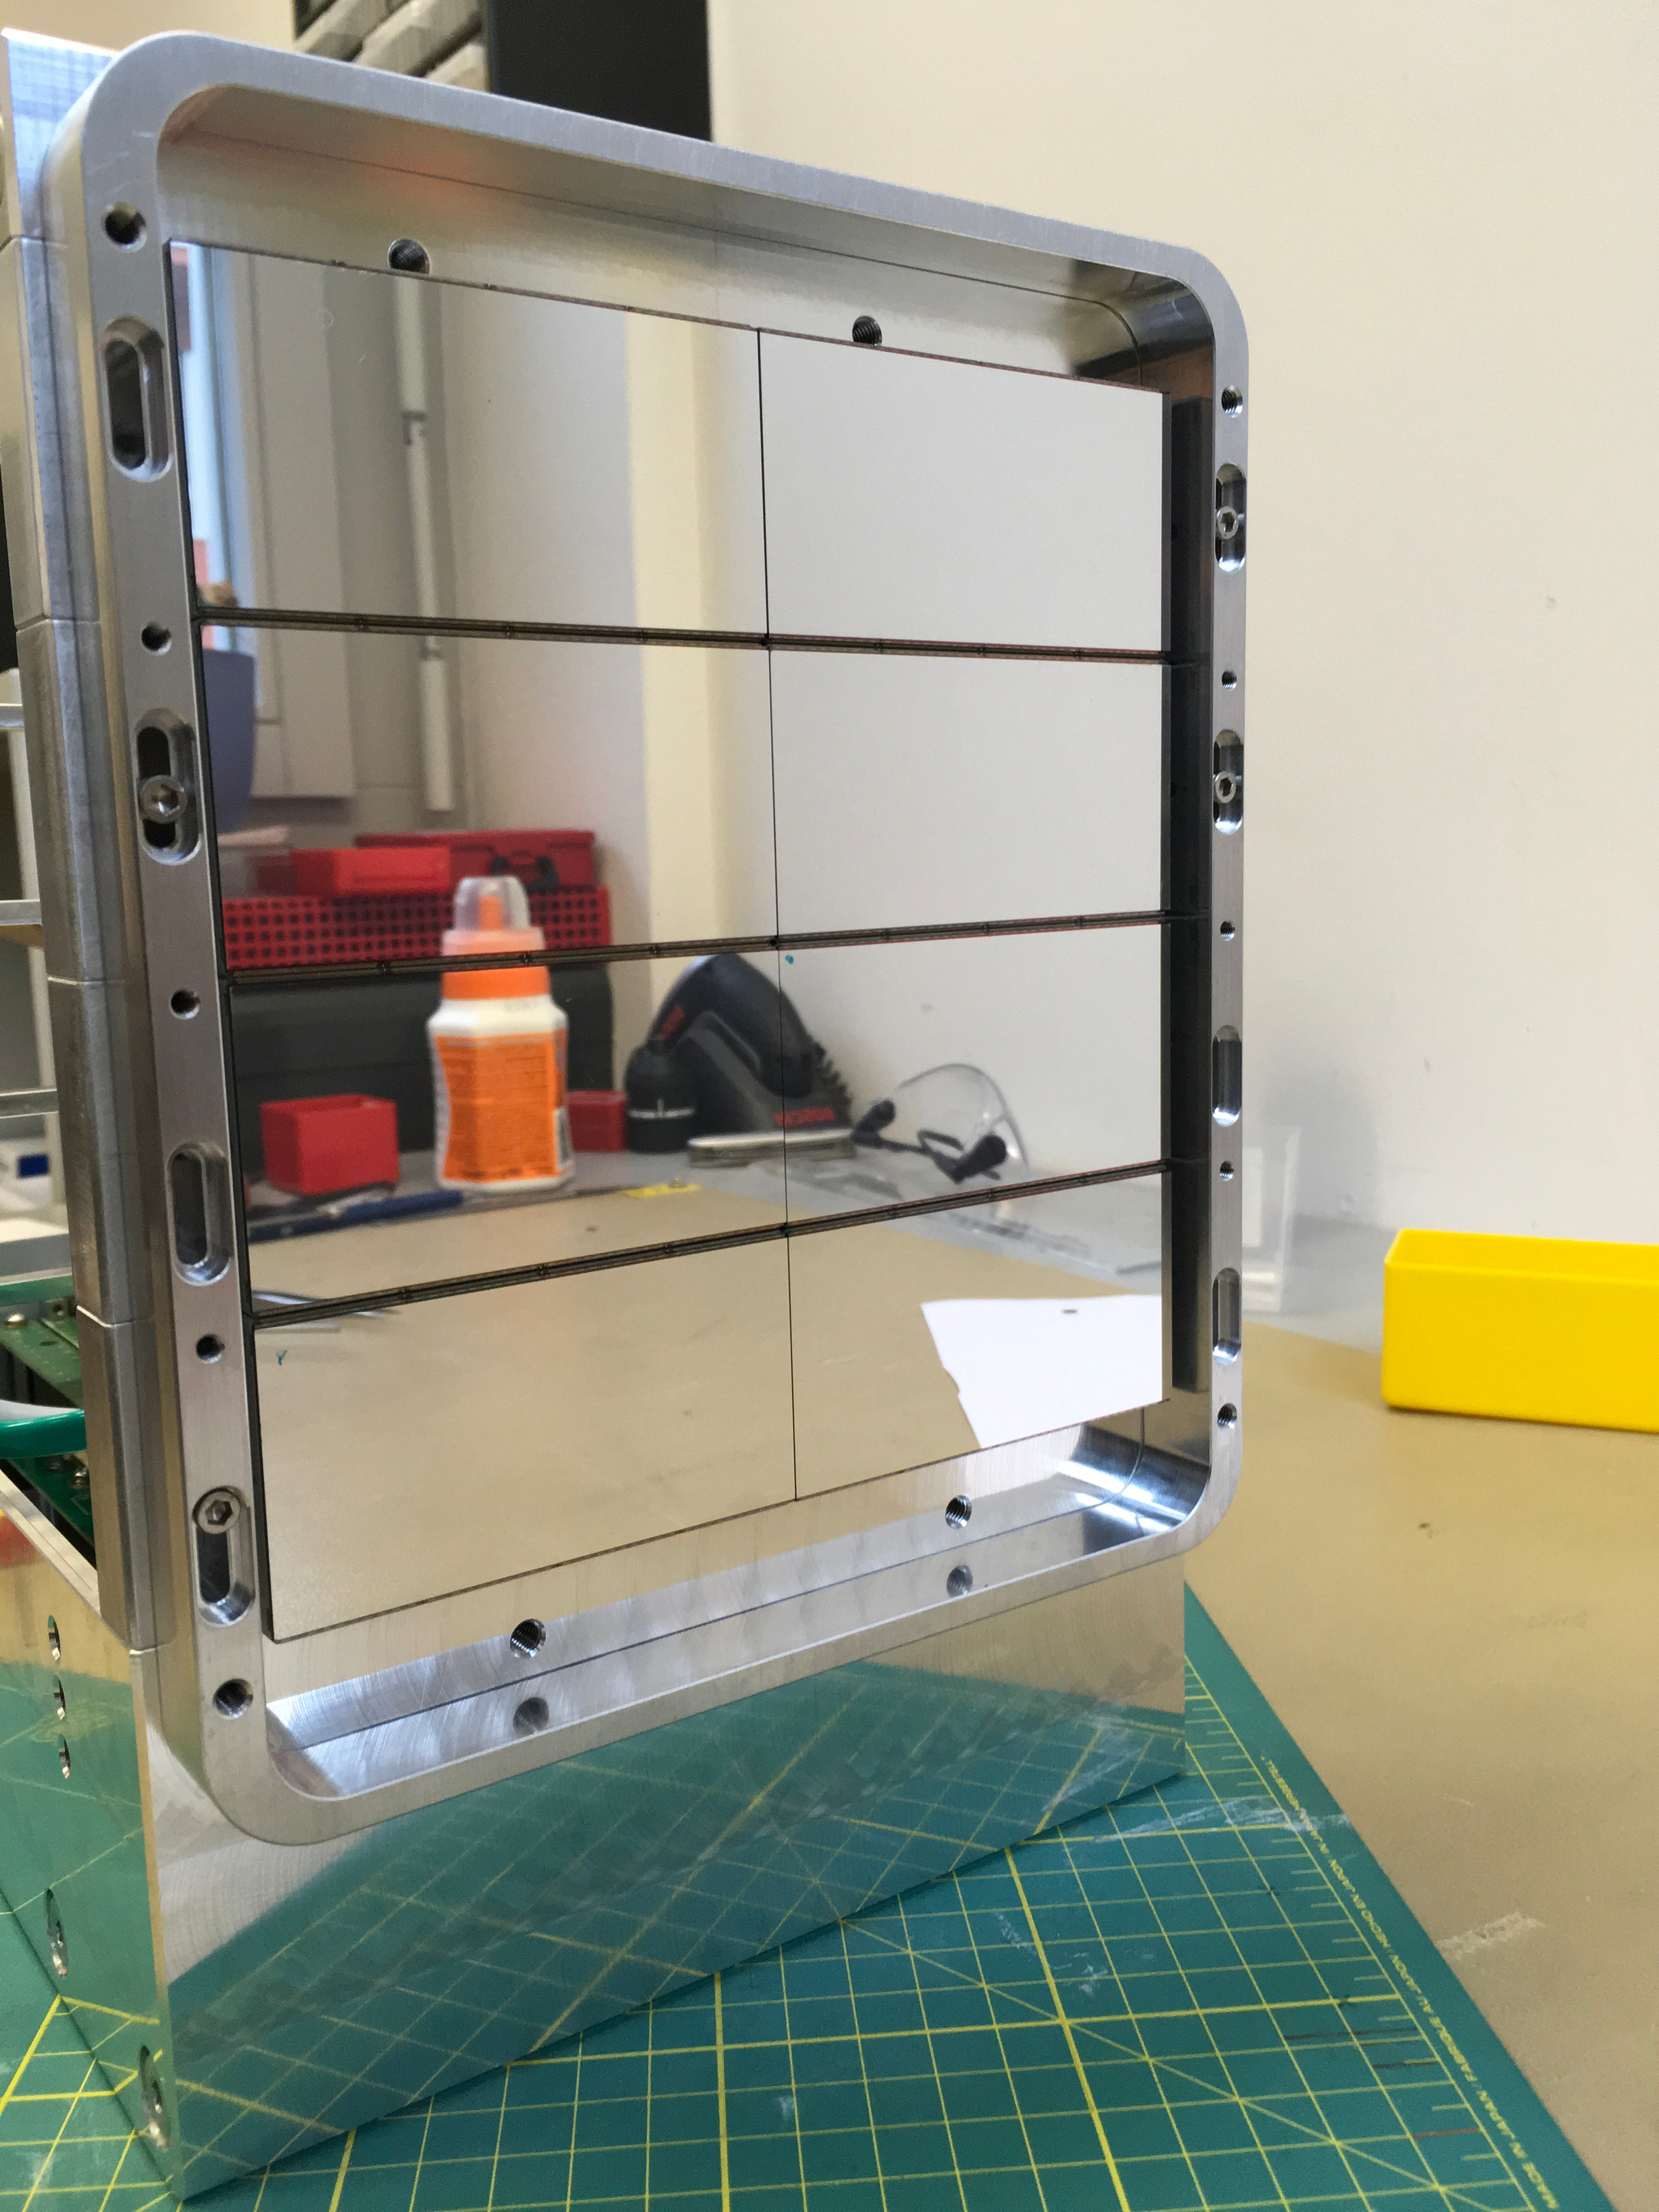
\includegraphics[width=0.30\textwidth]{jungfraudetector.jpg}
\caption{Jungfrau detector}
\label{fig:jfdetector}
\end{figure}


\subsection{Data processing algorithm (PSI)}
\label{subsec:alg}
conversion from detector data to energy and number of photons including pixel mask, pedestal calculation, pedestal tracking, pedestal correction, gain correction, conversion to number of photons (in the case of monochromatic incident radiation)\\

 summation of frames\\

 clustering (reference?)\\

\subsection{Alpaka implementation of fast data processing (Jonas, Florian)}
\label{subsec:alpaka}

\subsection{Benchmark tests (Jonas, Florian)}
\label{subsec:benchmark}
Design, objectives, and evaluation of tests

\section{Results}
\label{sec:results}
\subsection{Achieved improvements (Jonas)}
Results of tests of software parts on various computing hardware using suitable Alpaka backends\\

Where are the bottlenecks\\

Available capacity on GPUs\\

Best system

\subsection{Experiences from practical application of improved code (PSI)}
Application results

\section{Conclusions and Outlook}
\label{sec:conclusions}
Is presented method applicable / useful for other detectors, e.g. AGIPD? \\

calculation on FPGAs in the future


\section{Acknowledges}
The authors would like to thank  the Alpaka developers (\textcolor{blue}{names?})for their support.\\

This project has received funding from the European Union's Horizon 2020 research and innovation programme under grant agreement No 654220 (EUCALL).

\newpage

\begin{sloppypar}
\printbibliography
\end{sloppypar}
\end{document}
